% Practice Test 19 — Florida Edition
% Questions: 30 (23 MC + 7 SA)
% Generated by scripts/generate_practice_tests.py

\begin{practiceQuestion}{1-3-q01}{mc}
\begin{questionText}
What is the constant of proportionality ($k$) for the table below?

\begin{center}
\begin{tabular}{|c|c|}
\hline $x$ & $y$ \\ \hline $3$ & $12$ \\ $5$ & $20$ \\ $8$ & $32$ \\ \hline
\end{tabular}
\end{center}
\end{questionText}
\choiceA{$3$}
\choiceB{$4$}
\choiceC{$8$}
\choiceD{$12$}
\correctAnswer{B}
\explanation{$k = \frac{y}{x} = \frac{12}{3} = 4$. Check: $\frac{20}{5} = 4$ and $\frac{32}{8} = 4$.}
\end{practiceQuestion}

\begin{practiceQuestion}{1-6-q25}{sa}
\begin{questionText}
A truck delivers $540$ packages in $3$ trips. How many trips are needed to deliver $1{,}620$ packages?
\end{questionText}
\correctAnswer{$9$ trips}
\explanation{Per trip: $540 \div 3 = 180$ packages. Trips needed: $1{,}620 \div 180 = 9$.}
\end{practiceQuestion}

\begin{practiceQuestion}{2-1-q16}{mc}
\begin{questionText}
$9$ is $12\%$ of what number?
\end{questionText}
\choiceA{$1.08$}
\choiceB{$36$}
\choiceC{$72$}
\choiceD{$75$}
\correctAnswer{D}
\explanation{Divide the part by the percent: $9 \div 0.12 = 75$.}
\end{practiceQuestion}

\begin{practiceQuestion}{2-2-q22}{sa}
\begin{questionText}
A school garden has $80$ plants. If $45\%$ are tomato plants, how many tomato plants are there?
\end{questionText}
\correctAnswer{$36$}
\explanation{$\frac{n}{80} = \frac{45}{100}$. Cross-multiply: $100n = 3600$. Divide: $n = 36$ tomato plants.}
\end{practiceQuestion}

\begin{practiceQuestion}{2-6-q01}{mc}
\begin{questionText}
Find the simple interest: $P = \$500$, $r = 6\%$, $t = 3$ years.
\end{questionText}
\choiceA{$\$30$}
\choiceB{$\$60$}
\choiceC{$\$90$}
\choiceD{$\$150$}
\correctAnswer{C}
\explanation{$I = Prt = 500 \times 0.06 \times 3 = \$90$.}
\end{practiceQuestion}

\begin{practiceQuestion}{2-7-q03}{mc}
\begin{questionText}
In the percent error formula, why do we use absolute value?
\end{questionText}
\choiceA{To make the calculation easier}
\choiceB{Because the answer must be positive}
\choiceC{Because we only care about the size of the error, not the direction}
\choiceD{To convert the answer to a percent}
\correctAnswer{C}
\explanation{Absolute value ensures the percent error is positive whether the estimate was too high or too low.}
\end{practiceQuestion}

\begin{practiceQuestion}{3-2-q18}{mc}
\begin{questionText}
What value of $n$ makes $(-9) + n = -2$ true?
\end{questionText}
\choiceA{$-11$}
\choiceB{$-7$}
\choiceC{$7$}
\choiceD{$11$}
\correctAnswer{C}
\explanation{$(-9) + n = -2$ means $n = -2 - (-9) = -2 + 9 = 7$.}
\end{practiceQuestion}

\begin{practiceQuestion}{3-3-q21}{sa}
\begin{questionText}
Find the distance between $-11$ and $-3$ on a number line.
\end{questionText}
\correctAnswer{$8$ units}
\explanation{Distance $= |{-11} - (-3)| = |{-11} + 3| = |{-8}| = 8$ units.}
\end{practiceQuestion}

\begin{practiceQuestion}{4-4-q11}{mc}
\begin{questionText}
Factor $-12y + 8$.
\end{questionText}
\choiceA{$4(-3y + 2)$}
\choiceB{$-4(3y + 2)$}
\choiceC{$-4(3y - 2)$}
\choiceD{Both A and C}
\correctAnswer{D}
\explanation{$4(-3y + 2) = -12y + 8$ \checkmark. Also $-4(3y - 2) = -12y + 8$ \checkmark. Both are valid factored forms.}
\end{practiceQuestion}

\begin{practiceQuestion}{4-5-q02}{mc}
\begin{questionText}
Simplify $(6a - 2) - (3a + 5)$.
\end{questionText}
\choiceA{$3a + 3$}
\choiceB{$3a - 7$}
\choiceC{$9a - 7$}
\choiceD{$3a + 7$}
\correctAnswer{B}
\explanation{Distribute the negative: $6a - 2 - 3a - 5$. Combine: $(6a - 3a) + (-2 - 5) = 3a - 7$.}
\end{practiceQuestion}

\begin{practiceQuestion}{5-3-q12}{mc}
\begin{questionText}
Solve $7(x - 2) = 0$.
\end{questionText}
\choiceA{$x = 0$}
\choiceB{$x = -2$}
\choiceC{$x = 2$}
\choiceD{$x = 7$}
\correctAnswer{C}
\explanation{Divide by $7$: $x - 2 = 0$. Add $2$: $x = 2$. Check: $7(2 - 2) = 7(0) = 0$ \checkmark.}
\end{practiceQuestion}

\begin{practiceQuestion}{5-4-q21}{sa}
\begin{questionText}
Solve $\dfrac{x}{2} + \dfrac{x}{4} = 9$.
\end{questionText}
\correctAnswer{$x = 12$}
\explanation{Multiply every term by $4$: $2x + x = 36$. Combine: $3x = 36$. Divide by $3$: $x = 12$. Check: $\frac{12}{2} + \frac{12}{4} = 6 + 3 = 9$ \checkmark.}
\end{practiceQuestion}

\begin{practiceQuestion}{5-5-q27}{gmc}
\begin{questionText}
Look at the number line. Which inequality has this solution?

\begin{center}
\begin{tikzpicture}[scale=0.7]
  \draw[thick,->] (-6,0) -- (4,0);
  \foreach \x in {-5,...,3} \draw (\x,0.15) -- (\x,-0.15) node[below] {$\x$};
  \draw[thick,funOrange,<-] (-6,0) -- (-2,0);
  \fill[funOrange] (-2,0) circle (4pt);
\end{tikzpicture}
\end{center}
\end{questionText}
\choiceA{$3x + 1 > -5$}
\choiceB{$-4x \geq 8$}
\choiceC{$2x - 3 < -7$}
\choiceD{$x + 5 > 3$}
\correctAnswer{B}
\explanation{The graph shows $x \leq -2$ (closed circle, shading left). $-4x \geq 8$: divide by $-4$ and flip: $x \leq -2$ \checkmark.}
\end{practiceQuestion}

\begin{practiceQuestion}{5-6-q22}{sa}
\begin{questionText}
Solve $10 - 4x < 2$. Describe the graph.
\end{questionText}
\correctAnswer{$x > 2$; open circle at $2$, shade right}
\explanation{Subtract $10$: $-4x < -8$. Divide by $-4$ and flip: $x > 2$. Open circle at $2$, shade right.}
\end{practiceQuestion}

\begin{practiceQuestion}{6-2-q06}{mc}
\begin{questionText}
A map uses $1$ cm $= 20$ km. You redraw it at $1$ cm $= 10$ km. What happens to the drawing?
\end{questionText}
\choiceA{Every length is halved}
\choiceB{Every length stays the same}
\choiceC{Every length is doubled}
\choiceD{Every length is multiplied by $10$}
\correctAnswer{C}
\explanation{Scale ratio: $\frac{20}{10} = 2$. Every length on the new drawing is $2$ times the old one. The drawing gets bigger because each cm now represents fewer real km.}
\end{practiceQuestion}

\begin{practiceQuestion}{6-4-q28}{gmc}
\begin{questionText}
The diagram shows two triangles. Both have angles $30°$, $60°$, and $90°$, but different side lengths. What does this demonstrate?

\begin{center}
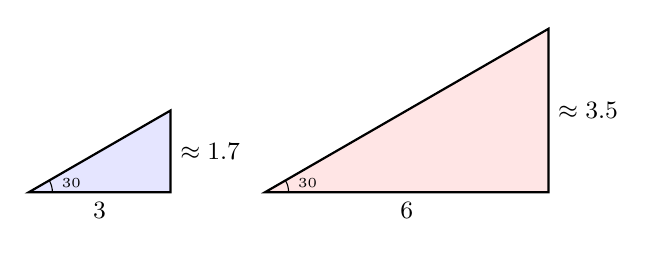
\begin{tikzpicture}[scale=0.6]
  % Small triangle
  \draw[thick,fill=blue!10] (0,0) -- (3,0) -- (3,1.73) -- cycle;
  \node[below] at (1.5,0) {\small $3$};
  \node[right] at (3,0.86) {\small $\approx 1.7$};
  \draw (0.5,0) arc[start angle=0,end angle=30,radius=0.5];
  \node at (0.9,0.2) {\tiny $30°$};
  % Large triangle
  \draw[thick,fill=red!10] (5,0) -- (11,0) -- (11,3.46) -- cycle;
  \node[below] at (8,0) {\small $6$};
  \node[right] at (11,1.73) {\small $\approx 3.5$};
  \draw (5.5,0) arc[start angle=0,end angle=30,radius=0.5];
  \node at (5.9,0.2) {\tiny $30°$};
\end{tikzpicture}
\end{center}
\end{questionText}
\choiceA{SSS produces multiple triangles}
\choiceB{AAA produces a unique triangle}
\choiceC{AAA produces multiple triangles of different sizes}
\choiceD{These two triangles are congruent}
\correctAnswer{C}
\explanation{Both triangles have the same angles but different side lengths. AAA determines shape but not size, so many triangles are possible.}
\end{practiceQuestion}

\begin{practiceQuestion}{6-5-q14}{mc}
\begin{questionText}
Which cross-section is NOT possible from slicing a rectangular prism?
\end{questionText}
\choiceA{Rectangle}
\choiceB{Triangle}
\choiceC{Circle}
\choiceD{Pentagon}
\correctAnswer{C}
\explanation{A rectangular prism has flat faces and straight edges. Its cross-sections can be triangles, rectangles, pentagons, or hexagons, but never circles (since it has no curved surfaces).}
\end{practiceQuestion}

\begin{practiceQuestion}{6-6-q13}{mc}
\begin{questionText}
Two lines intersect. One angle formed is $130°$. What are the measures of all four angles?
\end{questionText}
\choiceA{$130°$, $130°$, $50°$, $50°$}
\choiceB{$130°$, $50°$, $130°$, $100°$}
\choiceC{$130°$, $130°$, $130°$, $130°$}
\choiceD{$130°$, $60°$, $130°$, $40°$}
\correctAnswer{A}
\explanation{Vertical angles are equal ($130°$ and $130°$). Adjacent angles are supplementary: $180° - 130° = 50°$. The four angles are $130°$, $50°$, $130°$, $50°$.}
\end{practiceQuestion}

\begin{practiceQuestion}{7-1-q14}{mc}
\begin{questionText}
How many radii does it take to make one diameter?
\end{questionText}
\choiceA{$1$}
\choiceB{$2$}
\choiceC{$3$}
\choiceD{$4$}
\correctAnswer{B}
\explanation{A diameter is made up of two radii placed end to end through the center.}
\end{practiceQuestion}

\begin{practiceQuestion}{7-5-q09}{mc}
\begin{questionText}
A rectangular prism has dimensions $7$ m by $4$ m by $3$ m. What is the area of the largest face?
\end{questionText}
\choiceA{$12$ m$^2$}
\choiceB{$21$ m$^2$}
\choiceC{$28$ m$^2$}
\choiceD{$84$ m$^2$}
\correctAnswer{C}
\explanation{The three pairs of faces have areas $7 \times 4 = 28$, $7 \times 3 = 21$, and $4 \times 3 = 12$ m$^2$. The largest is $28$ m$^2$.}
\end{practiceQuestion}

\begin{practiceQuestion}{7-6-q04}{mc}
\begin{questionText}
A rectangular fish tank is $50$ cm long, $30$ cm wide, and $40$ cm tall. What is the volume?
\end{questionText}
\choiceA{$120$ cm$^3$}
\choiceB{$6{,}000$ cm$^3$}
\choiceC{$60{,}000$ cm$^3$}
\choiceD{$600$ cm$^3$}
\correctAnswer{C}
\explanation{$V = 50 \times 30 \times 40 = 60{,}000$ cm$^3$.}
\end{practiceQuestion}

\begin{practiceQuestion}{7-7-q09}{mc}
\begin{questionText}
What is the surface area of a cylinder with radius $3$ cm and height $7$ cm? Use $\pi \approx 3.14$.
\end{questionText}
\choiceA{$131.88$ cm$^2$}
\choiceB{$175.84$ cm$^2$}
\choiceC{$188.4$ cm$^2$}
\choiceD{$197.82$ cm$^2$}
\correctAnswer{C}
\explanation{$SA = 2\pi r^2 + 2\pi rh = 2(3.14)(9) + 2(3.14)(3)(7) = 56.52 + 131.88 = 188.4$ cm$^2$.}
\end{practiceQuestion}

\begin{practiceQuestion}{8-1-q27}{gmc}
\begin{questionText}
The diagram below shows four different sampling methods used to survey students at a school. Which method is most likely to produce an unbiased sample?

\begin{center}
\begin{tikzpicture}[scale=0.75]
  % Method A
  \node[draw,rounded corners,fill=funBlue!15,minimum width=3.5cm,minimum height=1.2cm,align=center] (A) at (0,3) {\textbf{Method A}\\Survey the football team};
  % Method B
  \node[draw,rounded corners,fill=funGreen!15,minimum width=3.5cm,minimum height=1.2cm,align=center] (B) at (6,3) {\textbf{Method B}\\Survey every 10th student\\on the school roster};
  % Method C
  \node[draw,rounded corners,fill=funOrange!15,minimum width=3.5cm,minimum height=1.2cm,align=center] (C) at (0,0) {\textbf{Method C}\\Post survey online and\\wait for responses};
  % Method D
  \node[draw,rounded corners,fill=funRed!15,minimum width=3.5cm,minimum height=1.2cm,align=center] (D) at (6,0) {\textbf{Method D}\\Survey students in\\one math class};
\end{tikzpicture}
\end{center}
\end{questionText}
\choiceA{Method A}
\choiceB{Method B}
\choiceC{Method C}
\choiceD{Method D}
\correctAnswer{B}
\explanation{Selecting every 10th student from the school roster is systematic and gives all students a chance, making it the least biased.}
\end{practiceQuestion}

\begin{practiceQuestion}{8-3-q22}{sa}
\begin{questionText}
Team A: mean $60$, MAD $4$. Team B: mean $70$, MAD $3$. Is the difference in means meaningful? Explain briefly.
\end{questionText}
\correctAnswer{Yes; the means are about $2.5$ to $3.3$ MADs apart}
\explanation{Difference $= 10$. Using MAD of $4$: $\frac{10}{4} = 2.5$. Using MAD of $3$: $\frac{10}{3} \approx 3.3$. Both are greater than $2$, so the difference is meaningful.}
\end{practiceQuestion}

\begin{practiceQuestion}{8-4-q03}{mc}
\begin{questionText}
Group A has a mean of $50$ and a MAD of $3$. Group B has a mean of $60$ and a MAD of $3$. The difference in means expressed in MADs is:
\end{questionText}
\choiceA{$\frac{10}{3} \approx 3.3$ MADs}
\choiceB{$10$ MADs}
\choiceC{$3$ MADs}
\choiceD{$30$ MADs}
\correctAnswer{A}
\explanation{Difference $= 60 - 50 = 10$. In MADs: $\frac{10}{3} \approx 3.3$.}
\end{practiceQuestion}

\begin{practiceQuestion}{8-5-q13}{mc}
\begin{questionText}
Data: $45, 48, 52, 55, 55, 58, 61, 63$. Which is the correct stem-and-leaf plot?
\end{questionText}
\choiceA{Stems: $4, 5, 6$; Row $4$: $5\;\;8$; Row $5$: $2\;\;5\;\;5\;\;8$; Row $6$: $1\;\;3$}
\choiceB{Stems: $4, 5, 6$; Row $4$: $5\;\;8$; Row $5$: $5\;\;5\;\;2\;\;8$; Row $6$: $3\;\;1$}
\choiceC{Stems: $45, 48, 52$; no leaves}
\choiceD{Stems: $4, 5$; Row $4$: $5\;\;8$; Row $5$: $2\;\;5\;\;5\;\;8\;\;1\;\;3$}
\correctAnswer{A}
\explanation{Stems are tens digits ($4, 5, 6$), leaves are ones digits listed in order. Only choice A has correct stems and ordered leaves.}
\end{practiceQuestion}

\begin{practiceQuestion}{8-6-q16}{mc}
\begin{questionText}
A student creates a circle graph with sectors of $100°$, $80°$, $60°$, and $100°$. Is this circle graph correct?
\end{questionText}
\choiceA{Yes — the sectors look reasonable}
\choiceB{No — the angles add to $340°$, not $360°$}
\choiceC{No — there are too many sectors}
\choiceD{Yes — all angles are less than $180°$}
\correctAnswer{B}
\explanation{$100 + 80 + 60 + 100 = 340°$, which is $20°$ short of $360°$. The graph is incorrect.}
\end{practiceQuestion}

\begin{practiceQuestion}{9-4-q07}{mc}
\begin{questionText}
A coin is weighted so that heads comes up $60\%$ of the time. What is the probability of tails?
\end{questionText}
\choiceA{$0.60$}
\choiceB{$0.50$}
\choiceC{$0.40$}
\choiceD{$0.30$}
\correctAnswer{C}
\explanation{$P(\text{tails}) = 1 - 0.60 = 0.40$. Since heads and tails have different probabilities, this is a non-uniform model.}
\end{practiceQuestion}

\begin{practiceQuestion}{9-6-q30}{gsa}
\begin{questionText}
Look at the tree diagram for flipping three coins. What is the probability of getting exactly $2$ tails? Write your answer as a fraction in simplest form.

\begin{center}
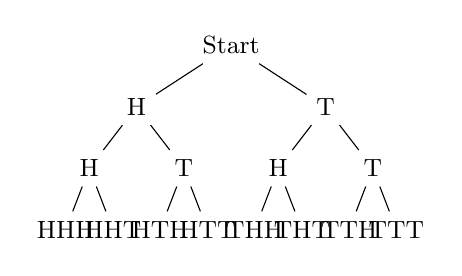
\begin{tikzpicture}[scale=0.6,
  level 1/.style={sibling distance=4cm, level distance=1.3cm},
  level 2/.style={sibling distance=2cm, level distance=1.3cm},
  level 3/.style={sibling distance=1cm, level distance=1.3cm}]
  \node {\small Start}
    child {node {\small H}
      child {node {\small H}
        child {node {\small HHH}}
        child {node {\small HHT}}
      }
      child {node {\small T}
        child {node {\small HTH}}
        child {node {\small HTT}}
      }
    }
    child {node {\small T}
      child {node {\small H}
        child {node {\small THH}}
        child {node {\small THT}}
      }
      child {node {\small T}
        child {node {\small TTH}}
        child {node {\small TTT}}
      }
    };
\end{tikzpicture}
\end{center}
\end{questionText}
\correctAnswer{$\frac{3}{8}$}
\explanation{Outcomes with exactly $2$ tails: HTT, THT, TTH — that is $3$ out of $8$. $P = \frac{3}{8}$.}
\end{practiceQuestion}

\begin{practiceQuestion}{9-7-q17}{mc}
\begin{questionText}
A student wants to simulate the probability that exactly $2$ out of $3$ students pass a test, where each student has a $50\%$ chance. Which model would work?
\end{questionText}
\choiceA{Roll one die: odd = pass, even = fail}
\choiceB{Flip $3$ coins: heads = pass, tails = fail; count exactly $2$ heads}
\choiceC{Draw $3$ marbles from a bag of $2$ red and $1$ blue}
\choiceD{Flip $1$ coin $3$ times and count all tails}
\correctAnswer{B}
\explanation{Each coin flip has a $50\%$ chance of heads (pass). Flipping $3$ coins and counting exactly $2$ heads simulates exactly $2$ passes.}
\end{practiceQuestion}
